In this thesis we research, find and describe a machine learning model for asset allocation. Asset allocation deals with the assignment of assets weights in an investment portfolio. This task and the finance studies field related to it is described in chapter \ref{CH:theoryFI}. The allocation produced by the model has to respect several requirements: it has a minimum and maximum investment exposition for each asset and it has to allow the user to have flexibility in maximizing the cumulative return while still maintaining volatility under a certain limit. We compared the allocation generated by the model against several benchmarks: a baseline algorithm based on components past Sharpe Ratio, equally weighted, inverse volatility and risk parity allocation methods. We achieved a higher cumulative return of the baseline algorithm and equally weighted in every validation period, while equal or better return of equally weighted or inverse volatility methods. The code generating these results is available on GitHub \footnote{\url{https://github.com/federicoB/Deep_Portfolio_Optimization}}.

\hfill \break

A proper assignment of weights can decide the success or failure of an investment plan. It is a relevant topic of research and numerous related works are published annually. Its complexity is intrinsic in the understanding on which assets are better to invest, therefore giving more weight. But financial markets are very complex systems. Price time series are non-linear, non-stationary, chaotic and noisy. In the seventies, efficient market hypothesis (EMH) was established by initial work of \textit{Malkiel and Fama (1970)} \cite{fama1970}, according to which financial markets follow random pathways and therefore are unpredictable. In more recent work, like the one of \textit{Kumar, Meghwani and Thakur (2016)} \cite{kumar2016}, there is evidence contrary to the efficiency of financial markets and the search for models and profitable systems is still attracting a lot of attention from academia. A predictive model capable of consistently generating returns above the market indices over time would represent strong evidence contrary to EMH. Fama himself, in a later work, revised his statement, indicating different levels of efficiency. 

\hfill \break

The challenges that a work like this thesis face are many: the selection of the best features to train the network, the selection of the best methods and architecture in a very extensive literature and making the network generalize better and perform well also out of sample. 

\hfill \break

As a machine learning model, we used neural networks, and specifically architectures made for sequence modelling tasks. Temporal Convolutional Networks (TCNs), Long Short Term Memory Networks (LSTMs) and Transformers were analyzed, used and compared. All these architectures layers and parameters are described in chapter \ref{CH:theoryML} and more implementation details can be found in chapter \ref{CH:Model_research}. We found out that TCNs were superior to the other two architectures both in terms of allocation quality and computational speed. Allocation quality can be defined both in term of high Sharpe Ratio or high cumulative return, it depends what the investor is looking for.


\hfill \break

Two different loss functions were analyzed, one inspired by the work of \textit{Zhang} (2020) \cite{zhang2019deep} computes the Sharpe Ratio of the portflio given the network output weights and aims to maximize it. This was very heavy computationally and did not showed relevant results so we moved to a second method. This second loss function is a mean squared error between the output weights and a target allocation generated a priori. This target allocation is generated knowing future returns and volatility in the training set. One important results of this thesis is that we show there is a correlation between target allocation parameters, i.e. return, Sharpe ratio and standard deviation, and the same parameters in the generated allocation. This means the network is learning to generate an allocation with the same characteristics of the allocation it was trained with. Furthermore and most important, this allow the user of the model to control risk.

\hfill \break

This work was done in collaboration with Salzenberg AI, an fintech company which provides trading signals for a managed investment fund. The fund trades four futures based on the Nasdaq100, Sp500, EuroSTOXX50 and Nikkei225 indices. My collaboration and internship was the search for a method based on machine learning for the allocation of capital between the four different assets. The model is not trained on returns of the Futures, but on \textit{strategy returns} over them. We create strategy returns for each of the 4 assets by multiplying the returns of a linked future with the values of a trading signal (see section \ref{s:trade_signal}). The trading signal is provided by Salzenberg AI, and is based on a proprietary strategy. Data available span from 2013 to 2020.


\hfill \break

The introduction continues doing a literature review on the subject. Chapter \ref{CH:theoryFI} and \ref{CH:theoryML} cover the background knowledge behind this work, on finance and machine learning respectively. Chapter \ref{CH:Model_research} delineates the methodology followed in this work and how we avoided some problems. Chapter \ref{CH:Results} shows all the results of the features and model selection. In the end, Chapter \ref{CH:Concl} recaps all the thesis work and describe possible future improvements. 

\section{Literature review}
\label{literature_review}

We introduce and briefly describe several recent works on the field of machine learning applied to asset allocation. This literature review by no means want to be exhaustive but want to give to the reader an idea of the different approaches that the research is following for solving this task.

The first work that has to be cited is the one of \textit{Snow (2020)} \cite{snow2020machine} as it is not directly an experiment but a formalization of the problem of asset allocation in many machine learning methods including regressions, autoencoders and reinforcement learning. Even if there are no experimental results but the formalization is clear and useful for a mathematical introduction in the field of machine learning for portfolio optimization.

\hfill \break

We then found other five works than can be subdivided either for the data used or the method applied. Three out of the five works use only historical assets prices like this thesis, while another one combined them with macro-economics indicators and another one with sentiments data. \\
Regarding the methods used, only one work tries to use Random Forest, two works use a Multi Layer Perceptron, two use Long-Short Term Memory Networks and other two use Reinforcement Learning.

\hfill \break

We first have to cite the work of \textit{Zhang et al. (2020)} \cite{Zhang_2020} as it was influential for this thesis and was the base from which we started. \\
Zhang developed a model that has the Sharpe ratio (see chapter \ref{CH:theoryFI}) as objective function to find the optimal portfolio weights using a LSTM Neural Network. 

As said by \textit{T{\"u}t{\"u}nc{\"u} (2006)} \cite{cornuejols2006optimization} optimizing Sharpe ratio by traditional means of quadratic programming is somewhat complicated as it is a non convex optimization problem. The traditional way would be reducing it to an equivalent problem, but machine learning can offer an alternative solution. \\


An interesting aspect of a machine learning solution to portfolio optimization is that it bypasses the step of forecasting the returns which are needed to apply Markowitz model. \\
Several works (\cite{moody2001learning, moody1998performance, zhang2019deep}) argue that the return forecasting methods does not guarantee that a portfolio's return will be maximized since the network optimizes a function targeting a more precise prediction on next day prices not next day portfolio performance.

\hfill \break

With this neural method, expected returns are not necessary, portfolio weights are computed directly from historical returns. This can be considered as an easier task for a neural network as it does not have to precisely predict the next daily price but an \textit{ordering} between the assets. Still, the quantitative difference between next day assets returns has to be implicitly predicted to decide how much to allocate on each.

\hfill \break

The architecture that Zhang uses is an LSTM with 50 units, followed by a fully connected layer and a softmax. The indices used are: US total stock index (VTI), US aggregate bond index (AGG), US commodity index (DBC) and Volatility Index (VIX). 
Results show as their model delivers the good performance in the testing period 2011-2020 as can be seen in figure \ref{fig:zhang_results}.

\begin{figure}
    \centering
    \floatbox[{\capbeside\thisfloatsetup{capbesideposition={left,top},capbesidewidth=4cm}}]{figure}[\FBwidth]
    {\caption[Zhang et.al (2020) results]{\textbf{Zhang et al. (2020) results}: cumulative returns. Allocation 1 is equal allocation, Allocation 2 is 50-10-20-20, Allocation 3 is 10-50-20-20, Allocation 4 is 40-40-10-10, MV means Mean-Variance optimization, MD means Maximum Diversification, DWP means Diversity weighted portoflio from Stochastic Portfolio Theory, DLS is Zhang model}
    \label{fig:zhang_results}}
    {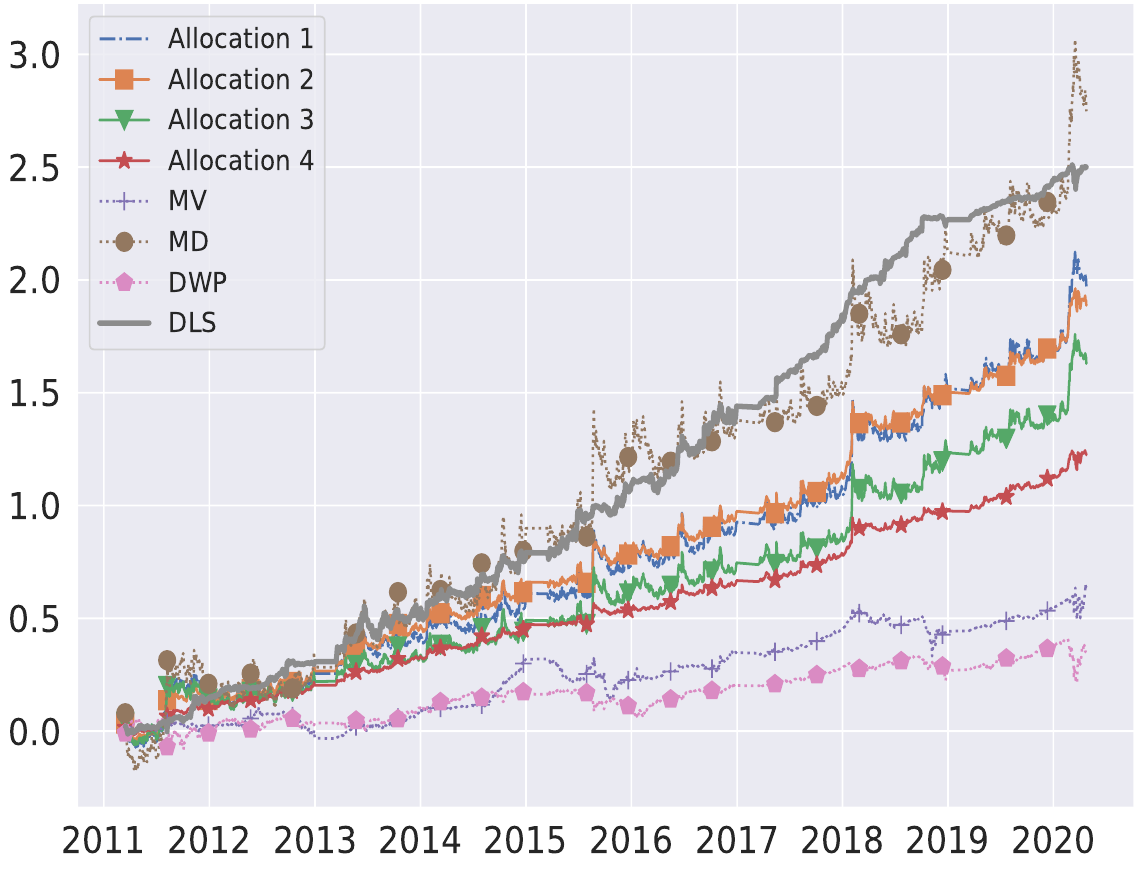
\includegraphics[width=10cm]{cap1/zhang_results.png}}

\end{figure}


A sensitive analysis is included to understand how input data contributes to outputs and the observation meet the econometric understating that most recent data is most relevant. Still this could be consequence of LSTM having problem to underline long term dependencies \cite{vaswani2017attention}.  

\hfill \break

Now two works that use Reinforcement Learning (RF). In finance, RF is particularly interesting as it tries to mimic human behaviour of searching for a reward and it is well know that the complex phenomenons observable in a financial markets are all the sum of many actors each trying to maximize their gains. Therefore, Reinforcement Learning could offer an appropriate way to model these agents behaviour.

\hfill \break

\textit{Wijs (2018)} \cite{weijs2018reinforcement} compare its reinforcement learning approach to portfolio optimisation with the one of \textit{Campbell (2002)}  \cite{campbell2002strategic} that use a Vector Autoregressive (VAR) model to forecast future returns. Wijs use 3 American assets: 3-month Treasure Bill, 5-year Treasury-Note and the weighted average of NYSE, NASDAQ and AMEX. Data spans a large period from 1954 to 2016. Results show a cumulative return of 33\% compared to Campbell method, a reduction of volatility of 33\% and a 3\% lower turnover.

\hfill \break

\textit{Kim (2020) } \cite{kim2020portfolio} is a very interesting work as it combines Reinforcement learning with Transformers. The reward is risk-adjusted as it includes the Sortino ratio. The agent uses a deep neural network, including Transformers layers, as a policy approximator. The model is trained and evaluated with assets of nine Dow Jones companies representing each sector. Data spans 20 years, from 2000 to 2020. The model takes sequences of 50 days. Results show a cumulative return over the years 2018 to 2020 of 43\% and an annualized Sharpe ratio of $0.64$.
Figure \ref{kim_results} and table \ref{tab:kim_results} summarize these results.

\begin{figure}[h]
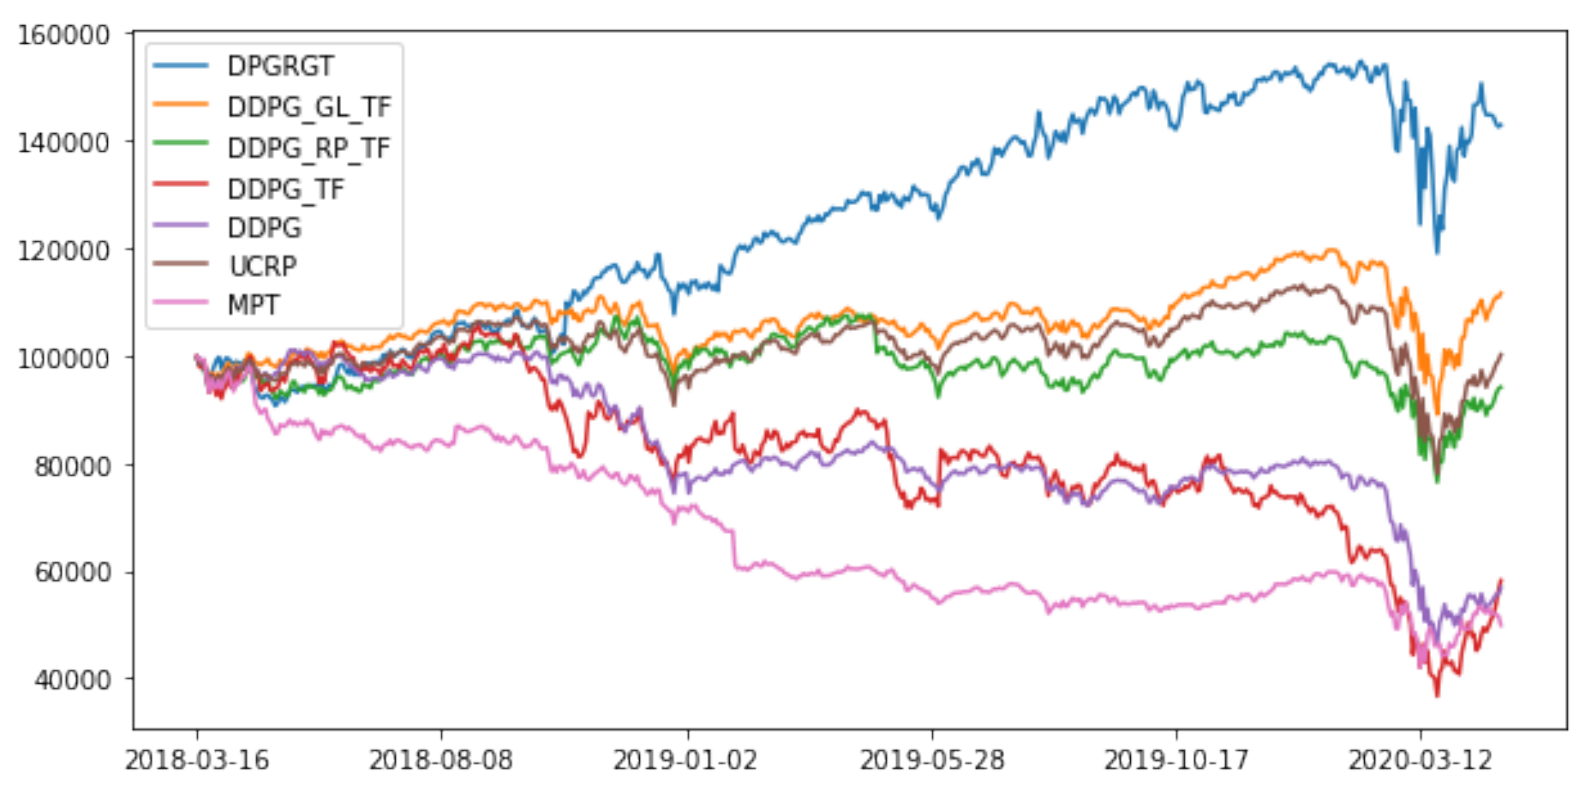
\includegraphics[width=12cm]{cap1/kim_results.png}
\caption[Kim (2020) results]{
\textbf{Kim (2020) results}: portfolio value after initial value of 10 thousand. MPT  is Markowitz’s Modern Portfolio Theory, UCRP is Uniform Constant Rebalanced Portfolio, DDPG stands from Deep Deterministic Policy Gradient and DDPG\_GL\_TF, DDPG\_RP\_TF, DDPG\_TF are DDPG  with Gated Transformer, Relative Attentional Transformer and standard Transformer respectively}
\label{kim_results}
\end{figure}

\begin{table}[h]
\begin{tabular}{|l|l|l|}
\hline
Model        & \begin{tabular}[c]{@{}l@{}}Cumulative\\ return (\%)\end{tabular} & \begin{tabular}[c]{@{}l@{}}Annualized\\ Sharpe Ratio\end{tabular} \\ \hline
DPGRGT       & 43.16                                                            & 0.6418                                                            \\ \hline
DDPG\_GL\_TF & 11.93                                                            & 0.2813                                                            \\ \hline
DDPG\_RP\_TF & -5.45                                                            & -0.1343                                                           \\ \hline
DDPG\_TF     & -41.71                                                           & -0.8191                                                           \\ \hline
DDPG         & -42.91                                                           & -1.2194                                                           \\ \hline
UCRP         & 0.53                                                             & 0.0125                                                            \\ \hline
MPT          & -50.07                                                           & -1.5840                                                           \\ \hline
\end{tabular}
\caption[Kim (2020) results]{ \label{tab:kim_results}
\textbf{Kim (2020) results}: cumulative return and annualized Sharpe Ratio. MPT  is Markowitz’s Modern Portfolio Theory, UCRP is Uniform Constant Rebalanced Portfolio, DDPG stands from Deep Deterministic Policy Gradient and DDPG\_GL\_TF, DDPG\_RP\_TF, DDPG\_TF are DDPG  with Gated Transformer, Relative Attentional Transformer and standard Transformer respectively}
\end{table}

\hfill \break

We now show two works where not only historical prices are used but macro-economics indicator and sentiment analysis are added to training data. While this makes the comparison with the previous works and the works in this thesis more difficult, it is interesting to examine these results as they can give an insight on what is can be reached with more type of data available.

\hfill \break

\textit{Chakravorty et al. (2018)} \cite{chakravorty2018deep} used price-volume  together with macroeconomics data in a feed-forward shrinking architecture for asset allocation. They use lagged returns over [260, 130, 60, 30] days partly to eliminate short term noise from the daily return and partly to keep turnover of the resulting investment strategy low.
The macro economics data used are US bond spread, Gold, Copper and Oil prices, US inflation, US non-farm job creation and US GDP growth. Two models were researched, one that forecasting expected returns and one directly computing weight by optimizing Sharpe ratio. 
The results performance are comparable to risk parity method (see Chapter \ref{CH:theoryFI})

\hfill \break

\textit{Malandri et. al (2018)} \cite{malandri2018public} add to historical price data, financial sentiment collected from Twitter, gaining better results than using only historical prices. It uses this data for training a model optimizing asset allocation in the New York Stock Exchange (NYSE). Historical prices are from 15 popular stocks. Sentiment data is the number of positive, negative, neutral comments and their daily change. They compare three different architectures: Multi layer perceptron, Random Forest and Long Short Term Memory network. Allocation is directly found by the network in an end-to-end fashion. The network is trained matching an allocation that allocates 100\% on the most remunerative asset. Finding shows how LSTM is superior with respect to the other two architectures. Unfortunately, the allocation performance is only compared against equally weighted portfolio. Still, it scores an increase in cumulative yearly return of 5\% without sentiment data and 19\% with.










